% ======================================================================

Este Capítulo descreve os dois conjuntos de dados que serão usados como
exemplos de aplicação no novo modelo de regressão, proposto no
\autoref{cap:multivariatemodel}. O primeiro conjunto se refere ao índice
de qualidade da água de reservatórios de usinas hidrelétricas operadas
pela COPEL no Estado do Paraná. Já o segundo conjunto de dados
corresponde ao percentual de gordura corporal de indivíduos avaliados no
Hospital de Clínicas da Universidade Federal do Paraná.

\section{CONJUNTO DE DADOS I: ÍNDICE DE QUALIDADE DA ÁGUA}
\label{cap:IQA}

\begin{table}[H]
  \centering
  \setlength{\abovecaptionskip}{.0001pt}
  \caption{ANÁLISE DESCRITIVA PARA O IQA POR TRIMESTRE E LOCAL}
  \label{tab:descIQA}
  \begin{tabular}{cccc}
    \hline
    \multirow{2}{*}{Trimestre} & \multicolumn{3}{c}{Local} \\
    \cline{2-4}  & Montante & Reservatório & Jusante \\
    \cline{2-4} 1   & $0,75\pm 0,11$   &  $0,80\pm 0,10$  &  $0,78\pm 0,10$  \\
    2  &  $0,79\pm 0,10$  &  $0,83\pm 0,06$   &  $0,83\pm 0,07$     \\
    3   &  $0,81\pm 0,07$   & $0,85\pm 0,05$   &  $0,83\pm 0,06$    \\
    4   & $0,76\pm 0,10$    &  $0,81\pm 0,08$    &  $0,79\pm 0,09$    \\
    \hline
  \end{tabular}
  \begin{footnotesize}
    \vspace{0.05cm}
    FONTE: O autor~(2018). \hspace{6.2cm}
    \vspace{-0.15cm}
  \end{footnotesize}
\end{table}

\vspace{-0.2cm}

\begin{figure}[H]
  \vspace{0.35cm}
  \setlength{\abovecaptionskip}{.0001pt}
  \caption{HISTOGRAMA~(A) E BOXPLOTS PARA O ÍNDICE DE QUALIDADE DA ÁGUA
    (IQA) POR TRIMESTRE~(B), LOCAL~(C) E USINAS~(D)}
  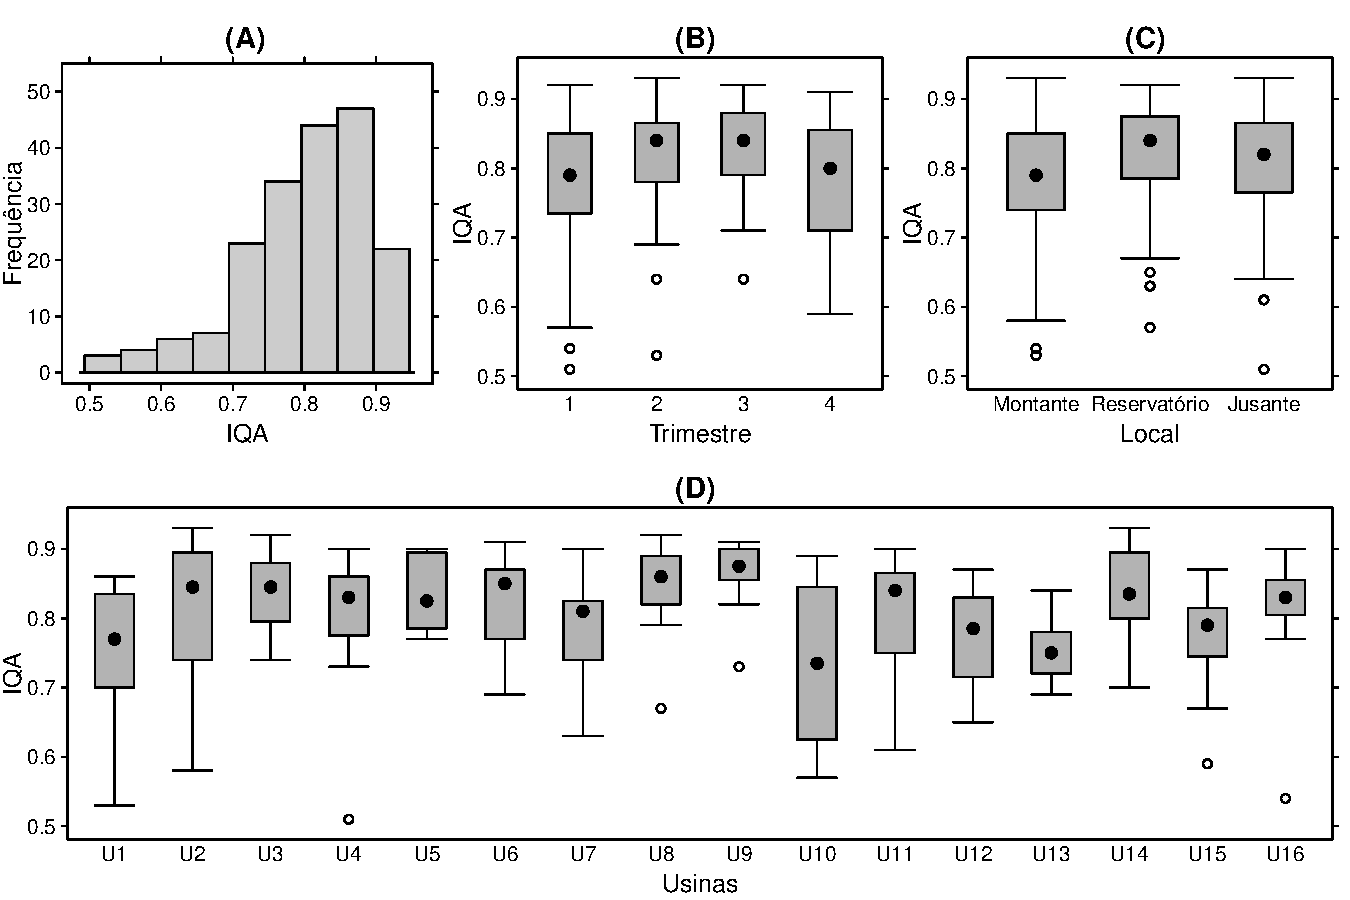
\includegraphics[width=0.95\textwidth]{Figure2.pdf}
  \begin{footnotesize}
    \vspace{-0.20cm}
    \centering
    FONTE: O autor~(2018).
    \vspace{0.15cm}
  \end{footnotesize}
  \label{fig:iqa1}
\end{figure}

Por fim, os resultados apresentados na~\autoref{fig:iqa1}~(D) mostram
que o IQA não é homogêneo entre as usinas, com um destaque maior para as
usinas 1, 2 e 10. É importante ressaltar que os resultados apresentados
na~\autoref{tab:descIQA} e~\autoref{fig:iqa1} se referem apenas a
análise descritiva e exploratória dos dados, onde são criadas hipóteses
que serão confirmadas somente após ajuste do modelo de regressão
proposto no~\autoref{cap:multivariatemodel}. No~\autoref{cap:apendiceA}
são apresentados gráficos boxplots para o IQA separado por trimestre e
local em função das usinas.

% ======================================================================